% $Id$
% ...........................................................................
%                  E L L I P T I S C H E  K U R V E N
% ~~~~~~~~~~~~~~~~~~~~~~~~~~~~~~~~~~~~~~~~~~~~~~~~~~~~~~~~~~~~~~~~~~~~~~~~~~~

\newpage
\section{Elliptic Curves}
\index{Elliptic curves}
\hypertarget{ellcurve}{}
(Filipovics B. / B\"uger M. / Esslinger B. / Oyono R., April 2000, Updates: Dec. 2001, June 2002, Mar. 2003)

\subsection{Elliptic curve cryptography -- a high-performance substitute for RSA?}\index{Performance}\label{ECAlternative}

In many business sectors secure and efficient data transfer is essential.
In particular, the RSA algorithm is used in many applications. Although the
security of RSA is beyond doubt, the evolution in computing power has
caused a growth in the necessary key length.  Today, 1024-bit RSA keys are
standard, but the GISA\index{GISA} (German Information Security Agency)
recommends the usage of 2048-bit keys from 2006 on (compare
section~\ref{SecurityRSA}).  The fact that most chips on smart cards cannot
process keys extending 1024 bit shows that there is a need for
alternatives. Elliptic curve cryptography (ECC) can be such an
alternative in the field of asymmetric cryptography.

The efficiency of a cryptographic algorithm depends on the key length and
the calculation effort that is necessary to provide a prescribed level of
security. The major advantage of ECC compared to RSA is that it requires
much shorter key lengths. If we assume that the computing power increases
by Moore's law (i.~e.\ it doubles every 18 months)\footnote{empirical
knowledge by Gordon Moore, co-founder of Intel, 1965}, then the evolution of
the key lengths for secure communication will be as figure~\ref{RSAKeylength}
\cite{Lenstra1999} (source: Arjen Lenstra and Eric Verheul:
\href{http://cryptosavvy.com/table.htm}
{\texttt{http://cryptosavvy.com/table.htm}}).

% -> Figure 1
\begin{figure}[h]
\begin{center}
\vspace{1.5cm}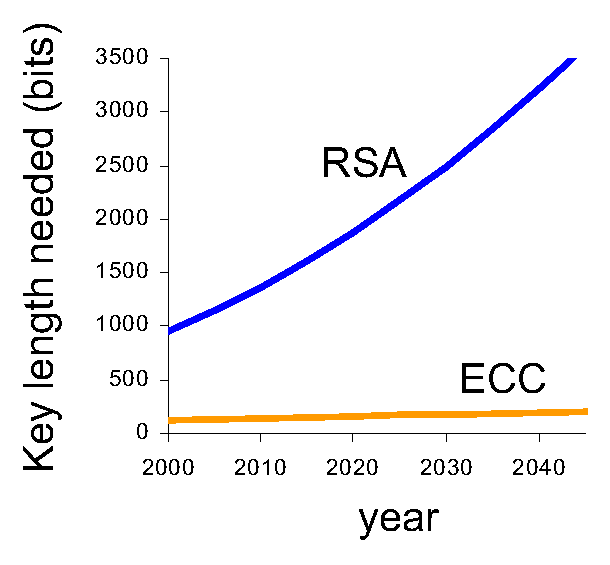
\includegraphics[scale=0.75]{figures/RSAKeylength}
\caption{Prognosis of the key lengths to be regarded safe for RSA and
  Elliptic Curves\vspace{1ex}} 
\label{RSAKeylength}
\end{center}
\end{figure}

In addition, a digital signature can be processed 10-times faster with ECC
than with RSA.  However, verification of a given signature is still more
efficient with RSA than with ECC. Refer to
figure~\ref{ThousandBitMultiplications} (source: Dr.~J.\ Merkle, Elliptic
Curve Cryptography Workshop, 2001) for a comparison.  The reason is that
RSA public keys can be chosen relatively small as long as the secret key is
long enough.

% -> Figure 2
\begin{figure}[h]
\begin{center}
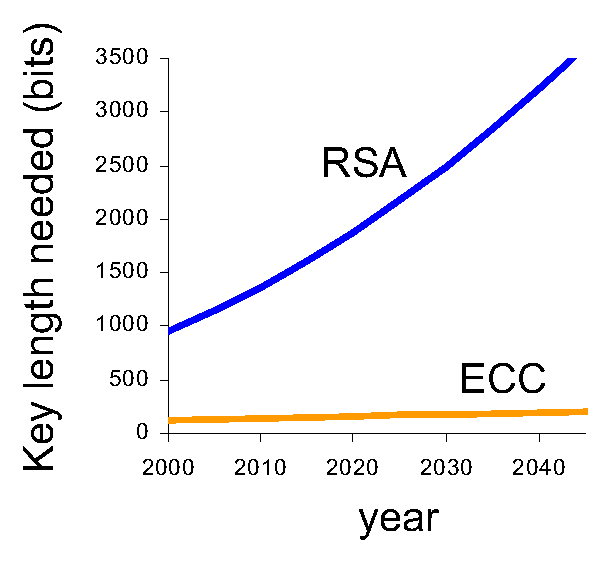
\includegraphics[scale=0.75]{figures/ThousandBitMultiplications}
\caption{Comparison of signing and verification time for RSA and Elliptic Curves} 
\label{ThousandBitMultiplications}
\end{center}
\end{figure}

Nevertheless, thin clients like smart cards usually have to store the (long)
secret key and have to process a digital signature rather than verify one.
Therefore, there is a clear advantage in using ECC in terms of efficiency.
\par
\smallskip
Nowadays, the major problem with ECC-implementations is the lack of standardization.
There is only one way to implement RSA, but there are many ways for ECC: One can work with
different sets of numbers, different (elliptic) curves --- described by parameters\footnote{%
see chapter \ref{ECC-Crypto}
} --- ,
and a variety of representations of the elements on the curve. Each choice has its
advantages and disadvantages, and one can certainly construct the most efficient for
each application. However, this causes problems in interoperability. But if all
ECC-tools should be able to communicate with each other, they will have to support
all different algorithms, which might put the advantage of efficient computation and
the need of less storage capacity to the contrary.

Therefore, international standardization organizations like IEEE (P1363),
ASC (ANSI X9.62, X9.63), ISO/IEC as well as major players like RSA labs or
Certicom have recently started standardization initiatives. While the IEEE
only describes the different implementations, the ASC has explicitly stated
10 elliptic curves and recommends their usage. The advantage of the ASC
approach is that one needs only a single byte to indicate which curve is
meant. However, it is not yet clear whether the ASC-curves will become a de
facto standard.

Although we see no need to replace RSA in any application today\footnote{%
Current informationen about the security of the RSA algorithm can be found in 
chapter \ref{SecurityRSA}.}, one should
take the usage of ECC-based tools into consideration whenever a new system
is set up --- in particular, when the tool should be available beyond 2005\footnote{%
Compare the recommendation of GISA: ``Fitting Crypto Algorithms'' from October 24th, 2002.
}.


\subsection{Elliptic curves -- history}

Mathematicians have been researching elliptic curves for over 100 years.
Over the course of time, many lengthy and mathematically complex results
have been found and published which are connected to elliptic curves. 
A mathematician would say that elliptic curves (or the mathematics behind
them) are widely understood. This research was originally purely 
mathematical. That is to say, elliptic curves were investigated, for 
example, in the mathematical areas of number theory and algebraic 
geometry, which are generally highly abstract. Even in the recent
past, elliptic curves played an important role in pure mathematics.
In 1993 and 1994, Andrew Wiles\index{Wiles Andrew} published 
mathematical works that triggered enthusiasm far beyond the specialist
audience. In these works, he proved a conjecture put forward in the 1960's.
To put it short, this conjecture was concerned with the connection 
between elliptic curves and what are called module forms. What is
particularly interesting for most people is that the works of Wiles
also proved the famous second theorem of Fermat. Mathematicians had
spent centuries (Fermat lived from 1601 to 1665) trying to find a
strict proof of this theorem. Understandably, therefore, Wiles' proof
got a good response. Fermat formulated his theorem as follows 
(written in the border of a book):

\begin{quote} {\em
Cubum autem in duos cubos, aut quadratoquadratum in duos quadratoquadratos, et
generaliter nullam in infinitum ultra quadratum potestatem in duos ejusdem
nominis fas est dividere: cujus rei demonstrationem mirabilem sane detexi. Hanc
marginis exiguitas non caperet.
} \end{quote}

With a free translation, using the denotation of modern mathematics, this means: \\
No positive whole numbers $x, y$ and $z$ greater than zero exist such that $x^n +y^n = z^n$ for $n>2$. I have found an amazing proof of this fact, but there is
too little space within the confines of this book to include it.

This is truly amazing: A statement that is relatively simple to understand (we
are referring to Fermat's second theorem here) could only be proved after such a
long period of time, although Fermat himself claimed to have found a proof.
What's more, the proof found by Wiles is extremely extensive (all of Wiles
publications connected with the proof made up a book in themselves). This should
therefore make it obvious that elliptic curves are generally based on highly
complex mathematics.

Anyway that's enough about the role of elliptic curves in pure mathematics. In 1985 Neal
Koblitz and Victor Miller independently suggested using elliptic curves in
cryptography. Elliptic curves have thus also found a concrete practical
application. Another interesting field of application for elliptic curves is for
factorising whole numbers. (For example the RSA cryptography system is based on
the \index{Complexity} difficulty/complexity of finding prime factors of an
extremely large number.) In this area, procedures based on elliptic curves have
been investigated and partially used since 1987 (a study by H.W. Lenstra). There
are also prime number tests\index{Prime number!test} based on elliptic curves.

Elliptic curves are used differently in the various areas. Encryption
procedures based on elliptic curves are based on the difficulty of a problem
known as elliptic curve discrete logarithm\index{Logarithm problem!discrete}.
The factorisation of whole numbers uses the fact that a large number of
elliptic curves can be generated for a natural composite number $n$ with
several prime factors; however, these curves are not then groups for composite
$n$. More information about this can be found under the chapter \ref{faktell}.

\subsection{Elliptic curves -- mathematical basics}

This section provides information about \index{Group} {\em groups} and
\index{Field} {\em fields}.

\subsubsection{Groups}

Because the term {\em group} is used differently in everyday language than in
mathematics, we will, for reasons of completeness, begin by introducing the
essential statement of the formal definition of a group:
\begin{itemize}
   \item A group is a non-empty set $G$ on which an operation ``$\cdot$''. The set $G$ is closed under this operation, which means that for any two elements $a, b$ taken from $G$, performing the operation on them gives an element in $G$, i.e. $ab=a\cdot b$ lies in $G$.
   \item For all elements $a, b$ and $c$ in $G$: $(ab)c = a(bc)$ (associative law).
   \item There exists an element $e$ in $G$ that behaves neutrally with respect
to the operation $\cdot$. That means that for all a in the set $G: ~ae = ea = a$.
   \item For each element $a$ in $G$ there exists a so-called inverse\footnote{The inverse is uniquely determined because if $x,y\in G$ are each inverse to $a$, i.e. $ax=xa=e$ and $ay=ya=e$, then $x=xe=x(ay)=(xa)y=ey=y$.} element $a^{-1}$ in $G$ such that: $aa^{-1} = a^{-1}a = e$.
\end{itemize}
If also $ab = ba$ (commutative law) for all $a, b$ in $G$, then we call the group an {\em Abelian} group.

Since we may define different operations on the same set, we distinguish them by giving them different names (e.g. $+$ addition or $\cdot$ multiplication).

The simplest example of an (Abelian) group is the group of whole numbers under
the standard operation of addition. The set of whole numbers is denoted as
${\mathbb Z}$. ${\mathbb Z}$ has an infinite number of elements, because
${\mathbb Z} = \{ \cdots, -4, -3, -2, -1, 0, 1, 2, 3, 4, \cdots\}$. For example, the
operation of $1+2$ lies in ${\mathbb Z}$, for $1+2 = 3$ and $3$ lies in
${\mathbb Z}$. The neutral element in the group ${\mathbb Z}$ is $0$. The
inverse element of $3$ is $-3$, for $3+(-3) = 0$.

For our purpose, so-called {\em finite} groups play an important role. This means that these exists a set
$\mathcal{M}$ with a fixed number of elements and an operation $+$ such that the
above conditions are fulfilled. One example of this is any set ${\mathbb Z}_n$
where ${\mathbb Z}_n = \{0, 1, 2, 3, \cdots, n-1\}, n$ is a positive whole number
and the operation is addition mod $n$, i.e. $a$ and $b$ in ${\mathbb Z}_n$ are
subject to the operation $a+b \;{\rm mod~} n$.

\paragraph{Cyclic groups}\index{Group!cyclic}
Cyclic groups\footnote{Cyclic groups can be in general also endless like the additive group of the integer numbers. We consider here only finite cyclic groups.} are those groups $G'$ that possess an element $g$
from which the group operation can be used to generate all other
elements in the group. This means that for each element $a$ in
$G'$ there exists a positive whole number $i$ such that if $g$ is
subject to the operation $i$ times (i.e. ``$g\cdot i$''),
$g+g+\cdots+g = a$ (additive group) or $g^i = g\cdot g \cdots g = a$
(multiplicative group). The element $g$ is the {\em generator} of
the cyclic group --- each element in $G�$ can be generated using
$g$ and the operation.

\paragraph{Group order}
Now to the order of an element of the group: Let $a$ be in $G$. The smallest
positive whole number $r$ for which $a$ subject to the operation with itself $r$
times is the neutral element of the group $G�$ (i.e.: $r \cdot a = a+a+\cdots+a =
e$ respectively $a^r = e$), is called the {\em order} of $a$.

The order of the group is the number of elements in the set $G$.

\subsubsection{Fields}

In mathematics, one is often interested in sets on which at least two (group) operations are defined --- frequently called addition and multiplication. Most prominent are so called fields.

A field is understood to be a set $K$ with two operations
(denoted as $+$ and $\cdot$) which fulfils the following conditions:
\begin{itemize}
   \item The set $K$ forms an Abelian group together with the operation $+$
(addition), where $0$ is the neutral element of the operation $+$.
   \item The set $K\setminus\{ 0\}$ also forms an Abelian group
together with the operation $\cdot$ (multiplication).
   \item For all elements $a, b$ and $c$ in $K$, we have $c\cdot (a+b) = c \cdot a + c
\cdot b$ and $(a+b) \cdot c = a \cdot c + b \cdot c$ (distributive law).
\end{itemize}

Fields may contain an infinite number of elements (e.g. the field of real numbers). They are called {\em infinite} fields. In contrast we call a field
{\em finite}, if it contains only a finite number of elements (e.g. ${\mathbb Z}_p = \{0, 1, 2, 3, \cdots, p-1\}$
, where $p$ is a prime. ${\mathbb Z}_p$ with addition mod $p$ and multiplication
mod $p$).
\index{Field!Characteristic}
\paragraph{Characteristic of a field}
Let $K$ be a field and $1$ be the neutral element of $K$ with
respect to the multiplicative operation ``$\cdot$''. Then the characteristic of $K$ is said to be the order of $1$ with respect to the additive operation. This means that the characteristic of $K$ is the smallest positive integer $n$ such that
$$ \underbrace{1+1+\dots+1}_{\hbox{$n$ times}} =0 .
$$
If there is no such $n$, i.e. if $1+1+\dots+1\ne 0$ no matter how many $1$s we add, then we call $K$ a field
with characteristic $0$.

Thus, fields with characteristic $0$ are infinite since they contain the (pairwise distinct) elements $1$, $1+1$, $1+1+1$, \dots. On the other hand, fields with finite characteristic may by finite or infinite.

If the characteristic is finite, it has to be prime. This fact can easily be proved: Assume $n=pq$, $p,q<n$, is the characteristic of a field $K$. By definition of $n$, the elements $\bar p=\underbrace{1+1+\dots+1}_{\hbox{$p$ times}}$, $\bar q=\underbrace{1+1+\dots+1}_{\hbox{$q$ times}}$ of $K$ are not equal to $0$. Thus, there exist inverse elements $\bar p^{-1},\bar q^{-1}$ with respect to multiplication. It follows that $(\bar p\bar q)(\bar p^{-1}\bar q^{-1})=1$, which contradicts the fact that $\bar p\bar q=\bar n=\underbrace{1+1+\dots+1}_{\hbox{$n$ times}}=0$ and, hence, $\underbrace{(\bar p\bar q)}_{=0}(\bar p^{-1}\bar q^{-1})=0$.

Comment: The field of real
numbers has the characteristic $0$; the field ${\mathbb Z}_p$ has
the characteristic $p$. If $p$ is not prime, ${\mathbb Z}_p$ is not a field at all.

The most simple field is ${\mathbb Z}_2=\{ 0,1\}$. It contains only two elements, the neutral elements with respect to addition and multiplication. In particular, we have $0+0=0$, $0+1=1+0=1$, $1+1=0$, $1\cdot 1=1$, $0\cdot 0=0\cdot 1=1\cdot 0=0$.

\index{Finite!Fields}
\paragraph{Finite Fields}
As mentioned above, each finite field has a characteristic $p\ne 0$, where $p$ is a prime. On the other hand, given a prime $p$ there is a field which has exactly $p$ elements, that is ${\mathbb Z}_p$.

However, the number of elements of a field need not be prime in general. For example, it is not hard to construct a field with $4$ elements\footnote{%
The set $K=\{0,1,a,b\}$ fitted with the operation defined in the tabular below is a field:\\
$
\begin{array}{|c||c|c|c|c|} 
\hline 
+ & 0 & 1 & a & b \\
\hline \hline
0 & 0 & 1 & a & b \\
\hline 
1 & 1 & 0 & b & a \\
\hline 
a & a & b & 0 & 1 \\
\hline 
b & b & a & 1 & 0 \\
\hline 
\end{array} \qquad {\rm ~und~} \qquad
\begin{array}{|c||c|c|c|c|} 
\hline 
\cdot & 0 & 1 & a & b  \\
\hline \hline
0 & 0 & 0 & 0 & 0 \\ 
\hline 
1 & 0 & 1 & a & b \\ 
\hline 
a & 0 & a & b & 1 \\ 
\hline 
b & 0 & b & 1 & a \\
\hline 
\end{array} 
$  \\
}.

One can show that the order of any field is a prime power (i.e. the power of a prime number). On the other hand, we can construct a field with $p^n$ elements for any given prime $p$ and positive integer $n$. Since two fields that have the same number of elements can not be distinguished\footnote{If $K,K'$ are fields with $k=p^n$ elements, then there is a one-to-one map $\varphi:K\to K'$, that respects the arithmetic of the field. Such a map is called an isomorphy. Isomorphic fields mathematically behave in the same way so that dass it makes no sense to distinguish between them. For example, ${\mathbb Z}_2$ und $K'=\{ ZERO,ONE\}$ with zero-element $ZERO$ and one-element $ONE$ are isomorphic. We note that mathematical objects are only defined by their mathematical properties.}, we say that there is {\bf the field with $p^n$ elements} and denote it by $GF(p^n)$. Here $GF$ stands for {\it Galois Field} to commemorate the French Mathematician Galois.

The fields $GF(p)$ of prime order play a prominent role. They are called prime fields and often denoted by ${\mathbb Z}_p$\footnote{For prime fields additive as well as multiplicative group are cyclic. Furthermore, each field $GF(p^n)$ contains a subfield that is isomorphic to the prime field ${\mathbb Z}_p$.}.



% -----------------------------------------------------------------------------
\subsection{Elliptic curves in cryptography}\label{ECC-Crypto}

In cryptography elliptic curve are a useful tool. Such curves are described by some equation. A detailed analysis has shown that curves of the form\footnote{This curve is given by the zeros of a {\it polynomial}\index{Polynomial} $F$ of degree three in three variables. In general, expressions of the form
$P=\sum_{i_1,\dots,i_n\in\N_0} a_{i_1\dots i_n} x_1^{i_1}\dots x_n^{i_n}$ with coefficients $a_{i_1\dots i_n}\in K$ are called polynomials in $n$ variables $x_1,\dots,x_n$ with underlying field $K$, if ${\rm deg\,} P:=\max\{i_1+\dots +i_n: a_{i_1\dots i_n}\ne 0\}$ is finite, i.e. the sum has only finitely many non-zero terms (monomials). The sum of the exponents of the variables of each term of the sum is at most $3$, at least one term of the sum has a single variable with $3$ as value of the according exponent.}
\begin{equation}
 F(x_1,x_2,x_3)=-x_1^3+x_2^2x_3+a_1x_1x_2x_3-a_2x_1^2x_3+a_3x_2x_3^2-a_4x_1x_3^2-a_6x_3^3=0,
\label{eccbasisgleichung}
\end{equation}
are especially useful. The variables $x_1,x_2,x_3$ and parameters $a_1,\dots,a_4,a_6$ are elements of a given field $K$, which has certain properties that are make it useful from the cryptographic point of view. The underlying field $K$ might be the well known field of real numbers or some finite field (see last section).
In order to obtain a cure that is useful for cryptography, the parameters have to be chosen in a way that the following conditions hold
$$ {\partial F\over\partial x_1}\ne 0, \quad {\partial F\over\partial x_2}\ne 0, \quad
{\partial F\over\partial x_3}\ne 0 .
$$
We identify points on the curve that can be derived from each over by multiplying each component with some scalar. This makes sense since $(x_1,x_2,x_3)$ solves (\ref{eccbasisgleichung}) if and only if $\alpha (x_1,x_2,x_3)$ ($\alpha\ne 0$) does. Formally, this means that we consider classes of equivalent points instead of single points, where points are called equivalent if one is the scalar multiple of the other one.
\\ If we put $x_3=0$ in the basic equation (\ref{eccbasisgleichung}), then this equation collapses to $-x_1^3=0$, leading to $x_1=0$. Thus, the equivalence class which includes the element $(0,1,0)$ is the only one that contains a point with $x_3=0$. For all points on the curve that are not equivalent to $(0,1,0)$, we may apply the following transformation
$$ K\times K\times (K\setminus\{0\})\ni (x_1,x_2,x_3) \mapsto (x,y):=\left( {x_1\over x_3}, {x_2\over x_3}\right) \in K\times K \, ,
$$
which reduces the number of variables to two instead of three. We note that the
basic equation (\ref{eccbasisgleichung}) $F(x_1,x_2,x_3)=0$  was chosen in a
way that this transformation leads to the famous so-called
Weierstrass-Equation\footnote{Karl Weierstrass\index{Weierstrass, Karl}, 31.10.1815$-$19.12.1897, German
mathematician, famous for his rigorous formal approach to mathematics.} holds
\begin{equation}
 y^2+a_1xy+a_3y = x^3+a_2x^2+a_4x+a_6 \, .
\label{ell}
\end{equation}
Since all but one point (i.e. equivalence class) of the elliptic curve can be described using equation (\ref{ell}), this equation is often called the elliptic equation, and its solutions written as
$$ {\bf E} = \left\{(x,y)\in K\times K \, |\, y^2+a_1xy+a_3y = x^3+a_2x^2+a_4x+a_6  \right\} \cup \{{\cal O} \}.
$$
Here, ${\cal O}$ represents the point $(0,1,0)$ that is loosely speaking mapped to infinity by the transformation (division by $x_3$) that reduces the three variables to two.

\begin{figure}[h]
\begin{center}
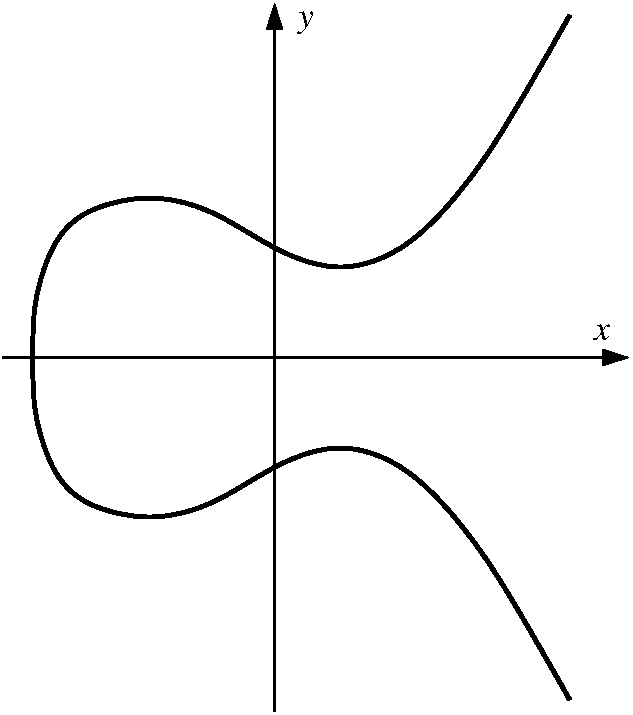
\includegraphics[scale=0.60]{figures/elliptic-curve}
\caption{Example of an elliptic curve with the real numbers as underlying field.\vspace{1ex}} 
\label{ExampleEllipticCurve}
\end{center}
\vskip -10 pt
\end{figure}

In contrast to figure \ref{ExampleEllipticCurve} only finite fields $K=GF(p^n)$ are used in elliptic curve cryptography. The reason is loosely speaking that in modern communication engineering data processing is always based on discrete data (simply because computers accept only discrete data).

For practical reasons, it turned out to be useful to take either $GF(p)$ with a large prime $p$ or $GF(2^n)$ with a (large) positive integer $n$. Using $GF(p)$ has the advantage of providing a relatively simple arithmetic; on the other hand $GF(2^n)$ allows a binary representation of each element that supports the way computers work. Other fields like, for example, $GF(7^n)$ do not have any of these advantages and are, thus, not considered, although there is no mathematical reason why they should not.

A coordinate transformation can result in a simpler version\footnote{Such a coordinate transformation is combination of a rotation and a dilatation of the coordinate system without changing the elliptic curve itself.} of the Weierstrass equation\index{Weierstrass, Karl}. Depending whether $p>3$, different transformations are used, and we obtain
\begin{itemize}
\item in case of $GF(p)$, $p>3$, the elliptic curve equation of the form
\begin{equation}
 y^2 = x^3 + ax + b
\label{ellp}
\end{equation}
with $4a^3+27b^2\ne 0$
\item in case of $GF(2^n)$ the elliptic curve equation of the form 
\begin{equation}
 y^2+xy = x^3 + ax^2 + b
\label{ell2}
\end{equation}
with $b\ne 0$\footnote{The form (\ref{ellp}) is called the standard form of the Weierstrass-equation\index{Weierstrass, Karl}. If the characteristic of the field is $2$ or $3$, we obtain $4=0$ respectively $27=0$, which means that the condition on parameters $a,b$ collapse. Loosely speaking, this is the reason why the transformation to the standard form does not work in these cases.}.
\end{itemize}
This conditions on the parameters $a,b$ ensure that the elliptic equation can be used in the context of cryptography\footnote{Formally we call such curves non singular.}.

Let $|E|$ denote the number of elements of an elliptic curve $E$ given an underlying field $GF(k)$ (for practical reasons either $k=p$ with $p$ prim or $k=2^n$). Then Hasse's theorem\cite{Silverman1986} yields $| \, |E| - k-1\,| \le 2\cdot \sqrt{k}$. This Inequality is equivalent to $k+1 - 2\sqrt{k} < |E| < k+1+2\sqrt{k}$. In particular, this means that the number of elements of an elliptic curve is approximately $k$ (for large $k$). 

% -----------------------------------------------------------------------------
\subsection{Operating on the elliptic curve}

In order to work with elliptic curves in practice, we define an operation (often written in an additive way $+$) on the set of points on the curve. If we have a curve over the field $GF(p)$, we define the commutative operation $+$ by
\begin{enumerate}
\item $P+{\cal O}={\cal O}+P=P$ for all $P\in E$,
\item for $P=(x,y)$ and $Q=(x,-y)$ we set $P+Q={\cal O}$,
\item for $P_1=(x_1,x_2),P_2=(x_2,y_2)\in E$ with $P_1,P_2\ne {\cal O}$ and $(x_2,y_2)\ne (x_1,-y_1)$ we set $P_3:=P_1+P_2$, $P_3=(x_3,y_3)$ defined by
$$ x_3:=-x_1-x_2+\lambda^2 \, , \qquad y_3:=-y_1+\lambda (x_1-x_3)
$$
with the auxiliary quotient
$$ \lambda:=\left\{ \begin{array}{cl} {y_1-y_2\over x_1-x_2} & {\rm if~} P_1\ne P_2, \\
                                     {3x_1^2+a\over 2y_1} & {\rm if~} P_1=P_2. \end{array} \right.
$$
\end{enumerate}
In particular, we obtain $-P=(x,-y)$ for $P=(x,y)\in E$.

If we deal with a curve over the field $GF(2^n)$, we define the operation $+$ in an analogous way by
\begin{enumerate}
\item $P+{\cal O}={\cal O}+P=P$ for all $P\in E$,
\item for $P=(x,y)$ and $Q=(x,x+y)$ we set $P+Q={\cal O}$,
\item for $P_1=(x_1,x_2),P_2=(x_2,y_2)\in E$ with $P_1,P_2\ne {\cal O}$ and $(x_2,y_2)\ne (x_1,x_1+y_1)$ we set $P_3:=P_1+P_2$, $P_3=(x_3,y_3)$ defined by
$$ x_3:=-x_1+x_2+\lambda+\lambda^2+a \, , \qquad y_3:=y_1+x_3+\lambda (x_1+x_3)
$$
with auxiliary quotient
$$ \lambda:=\left\{ \begin{array}{cl} {y_1+y_2\over x_1+x_2} & {\rm if~} P_1\ne P_2, \\
                                   x_1+{y_1\over x_1} & {\rm if~} P_1=P_2. \end{array}\right.
$$
\end{enumerate}
In particular, we obtain $-P=(x,-y)$ for $P=(x,y)\in E$.

(Note that $-(-P)=(x,x+(x+y))=(x,2x+y)=(x,y)$, since the underlying field has characteristic $2$.)\footnote{An animation of the addition of points on elliptic curves can be found on the Certicom\index{Certicom}-Homepage \\
\href{http://www.certicom.com/resources/ecc_tutorial/ecc_tutorial.html}{\texttt{http://www.certicom.com/resources/ecc\_tutorial/ecc\_tutorial.html}}}

One can verify that $+$ defines a group operation on the set $E\cap\{\cal O\}$.
In particular this means that the sum of two points is again a point on the
elliptic curve. How his operation works is geometrically visualized in the
following section.

% \newpage
\begin{figure}[htbp]
\subsubsection*{How to add points on an elliptic curve}
The following figures show how points on an elliptic curve over the field of real numbers are summed up using affine coordinates.
We note that the point infinity ${\cal O}$ cannot be shown in the affine plane.  
\begin{center}
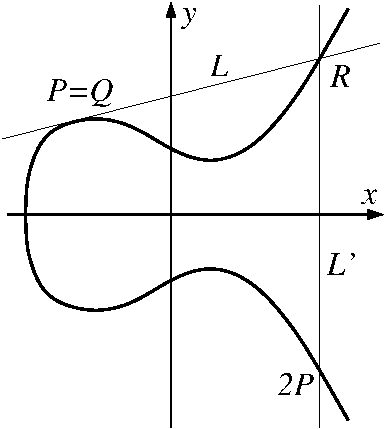
\includegraphics[scale=1.08]{figures/ec-mult2}
\caption{Doubling of a point} 
\vspace{\floatsep}
\vskip +20 pt
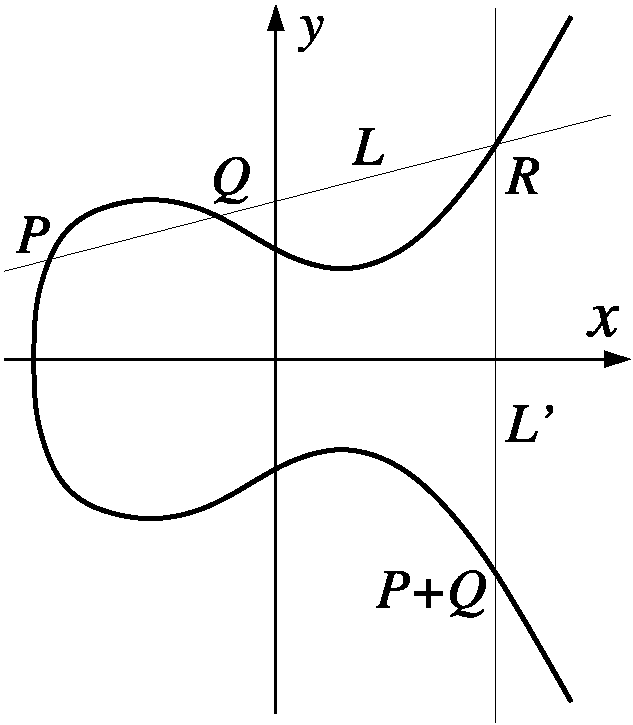
\includegraphics[scale=0.65]{figures/ec-add}
\caption{Summing up two different points over the real number field} % \footnotemark }
\end{center}
\end{figure}
\enlargethispage{+20pt}
\newpage


% -----------------------------------------------------------------------------
\subsection{Security of elliptic-curve-cryptography: The ECDLP}

As mentioned above in section \ref{ECC-Crypto}, we only consider elliptic curves over the finite\footnote{Discrete in contrast to continuous.} fields $GF(2^n)$ or $GF(p)$ (for a large prime $p$). This means that all parameters that describe the curve are taken from this underlying field. If $E$ is an elliptic curve over such a field and $P$ is a point on the curve $E$, then we can derive for all positive integers $m$
$$ mP := \underbrace{P+P+\dots+P}_{\hbox{$m$ times}} \, .
$$
Looking on this operation from the cryptographic point of view, it turns out to be very interesting by the following reason: On the one hand one needs only $\log m$ operations to calculate $mP$ --- one simply has to calculate $P$, $2P$, $2^2P$, $2^3P$, \dots, write $m$ in a binary form and finally add all these multilples $2^kP$ of $P$ with respect to the binary representation of $m$ --- on the other hand it seems to be very hard to find $m$ given $P$ and $Q=mP$ on $E$. Of course, we may simply calculate $P,2P,3P,4P,5P,\dots$ and compare each of them with $Q$. But this will take as much as $m$ operations.

Yet there is no algorithm known that efficiently derives $m$ given $P$ and $G$. The best algorithms known so far need about $\sqrt{q}$ operations where $q$ is the (largest) prime factor of $p-1$, in case the underlying field is $GF(p)$; here $m$ should be between $1$ and $q$ liegen so that one needs at most $\log q$ operations to calculate $mP$. However, the quotient ${\sqrt{q}\over\log q}$ tends to $+\infty$ very fast for large $q$.

If we choose the parameters sufficiently large (for example, let $p$ be prime and at least $160$ bits long), an computer will easily be able to calculate $mP$ (in less than a second). The {\it inverse problem} however, to derive $m$ from $mP$ and $P$, can (still) not be solved in reasonable time.

This problem is known as the ``over Elliptic Curve Discrete Logarithm Problem'' (for short ECDLP\index{ECDLP}).

\vskip +5 pt

In elliptic curve cryptography we formally look at points on the elliptic curve as elements of a group with point addition $+$ as operation. Furthermore, we use only elliptic curves that have a sufficiently large number of points. However, in special cases curves may be weak and not useful due to other reasons. For such special cases the ECDLP can be much easier to solve than in the general case. This means that one has to look carefully at the parameters when choosing an elliptic curve for cryptographic applications.

Not useful for cryptography are {\em a-normal} (that are curves over ${\mathbb Z}_p$,
for which the set ${\bf E}$ consists of exactly $p$ elements) and {\em supersingular} curves (that are curves, for which the ECDLP can be reduced to the ``normal'' discrete logarithms in another, smaller finite field). This means that there are cryptographically useful and non-useful elliptic curves. Given the parameters $a$ and $b$, it is possible to determine whether a curve is useful or not. In many publications one can find parameters that turned out to be useful for cryptography. The open (scientific) discussion guarantees that these results take into account latest research.
\vskip +5 pt

Given a secure curve, the time that is needed to solve the ECDLP is strongly correlated with parameter $p$ in case $GF(p)$ respectively $n$ in case of $GF(2^n)$. The larger these parameters become, the more time an attacker needs to solve the ECDLP --- at least with the best algorithms known so far. Experts recommend bit-lengths of $200$ for $p$ for secure curves. A comparison with RSA modulus length shows why elliptic curves are so interesting for applications. We note that the computation effort for signing and encryption is closely related to the bit-length of the parameters. In addition the initiation process, i.e. the generation of the private-public-key-pair, becomes more complicated the larger $p$ is. Thus, one looks for the smallest parameters that still come along with the security required. It is remarkable that a length of $200$ bits for $p$ is sufficient to construct a {\em good} elliptic curve that is as secure as RSA with a $1024$ bit \index{RSA!Modulus} RSA-Modulus (as far as we know today). For short, the reason for this advantage of ECC lies in the fact that the best algorithms known for solving the ECDLP need exponential time while the best algorithms for factorizing are sub-exponential (number field sieve, quadratic sieve or factorizing with elliptic curves). Hence, the parameters for a cryptosystem that is based on the problem of {\em factorizing large integers} have to be larger than the parameters for a system based on ECDLP.


% -----------------------------------------------------------------------------
\subsection{Encryption and signing with elliptic curves}

\begin{sloppypar}
  The {\em elliptic curve discrete logarithm
    problem}\index{Problem of discrete logarithm} (ECDLP) \index{ECDLP} is the basis for elliptic curve cryptography. Based on this problem, there are different signature schemes. In order to apply one of these, we need:
\end{sloppypar}
\begin{itemize}
    \item An elliptic curve {\bf E} with an underlying field $GF(p^n)$.
    \item A prime $q\ne p$ and a point $G$ on the elliptic curve ${\bf E}$ with order $q$. This means that $qG={\cal O}$ and $rG\ne {\cal O}$ for all $r\in \{1,2,\dots,q-1\}$. Thus $q$ is a factor of the group order (i.e. the number of elements) $\#{\bf E}$ of $E$. Since $q$ is prime, $G$ generates a cyclic sub-group of ${\bf E}$ of order $q$.
\end{itemize}
The parameters mentioned are often called \index{Domain-Parameter} {\em Domain}-Parameter. They describe the elliptic curve ${\bf E}$ and the cyclic sub-group of ${\bf E}$ on which the signature scheme is based.

\par
%\smallskip
%{\bf Encryption:}
\subsubsection{Encryption}

Using elliptic curves one can construct a key exchange protocol based on the \hyperlink{DH-KeyExch}{Diffie-Hellman Protokoll} \index{Diffie-Hellman} (see chapter \ref{DH-KeyExch}). The key exchanged can be used for a subsequent symmetric encryption. We note that in contrast to RSA there is no pair of private and public key that can be used for encryption and decryption!

In the notation of elliptic curves, the Diffie-Hellman protocol reads as follows: First both partners (A und B) agree on a group $G$ and an integer $q$. Then they choose $r_A,r_B\in\{1,2,\dots,q-1\}$ at random, derive the points $R_A=r_AG$, $R_B=r_BG$ on the elliptic curve and exchange them (using an insecure channel). After that A easily obtains $R=r_AR_B$; B gets the same point ($R=r_Ar_B G$) by calculating $r_BR_A=r_Br_AG=r_Ar_BG=R$. We note that $R_A,R_B$ are easy to derive as long as $r_A$ respectively $r_B$ are known $G$. However, the inverse operation, to get $R_A$ respectively $R_B$ from $r_A$ respectively $r_B$ is hard.
\\ Using the best algorithms known so far, it is impossible for any attacker to obtain $R$ without knowing either $r_A$ or $r_B$ --- otherwise he would have to solve the ECDLP.

In order to prohibit a ``Man-in-the-middle"{}~attack, one may sign the values $G,q,R_A,R_B$ as described in chapter \ref{Impersonalisierungsattacke}.


\par
%\smallskip 
%{\bf Signing:}
\subsubsection{Signing}

Using the DSA signature scheme, one can proceed as follows: The signing party chooses a (non-trivial) number $s\in{\mathbb Z}_q$, which will be the private key, and publishes $q$, $G$ and $R=sG$. We note that $s$ cannot be obtained from $G$ and $R$ are not sufficient --- a fact on which the security of the signature scheme is based.

Given the message $m$, which should be signed, one first constructs a digital finger print using a hash-algorithm $h$ such that $h(m)$ has its values in $\{0,1,2,\dots, q-1\}$. Thus, $h(m)$ can be considered as an Element of ${\mathbb Z}_q$. Then the signing party chooses a random number $r\in{\mathbb Z}_q$ and derives $R=(r_1,r_2)=rG$. We note that the first component $r_1$ of $R$ is an element of $GF(p^n)$. This component will then be projected onto ${\mathbb Z}_q$, i.e. in case of $n=1$ it is interpreted as the remainder of an element of $\{0,1,\dots,p-1\}$ divided by $q$. This projection of $r_1$ onto ${\mathbb Z}_q$ is denoted by $\bar r_1$. Then one determines $x\in {\mathbb Z}_q$ such that
$$ rx-s\bar r_1-h(m)=0 .
$$
The triple $(m,r_1,x)$ is then published as the digital signature of message $m$.

\par
%\smallskip 
%{\bf Signature Verification:}
\subsubsection{Signature verification}

In order to verify a signature, one has to build $u_1=h(m)/x$, $u_2=\bar r_1/x$ (in ${\mathbb Z}_q$ and derive
$$ V=u_1G+u_2Q .
$$
Since we have $Q=sG$, the point $V=(v_1,v_2)$ satisfies $v_1=u_1+u_2s$. We note that this operations take place in the field $GF(p^n)$. The projection of $GF(p^n)$ on ${\mathbb Z}_q$ mentioned above should be chosen in such a way that $\bar v_1=u_1+u_2s$ is an element of ${\mathbb Z}_q$. Then it follows that
$$ \bar v_1=u_1+u_2s=h(m)/x+\bar r_1 s/x=(h(m)+\bar r_1s)/x=rx/x=r .
$$
Since $R=rG$, we obtain $\bar v_1=\bar r_1$, i.e. $R$ and $V$ coincide modulo the projection onto ${\mathbb Z}_q$.


% -----------------------------------------------------------------------------
\subsection{Factorization using elliptic curves}

\label{faktell}

There are factorization algorithms based on elliptic curves%
\footnote{In 1987 H.W. Lenstra published
a factorization algorithm, based on elliptic curves (see \cite{Lenstra1987}).
The biggest compound number currently factorised\index{Factorization!factoring records} with elliptic curves is 
the number $ 628^{59}-1, $ which has 55 decimal digits. It was
found Oct. 6th, 2001 by M. Izumi 
(See \hyperlink{Lenstra2}{ECMNET}\index{ECMNET}).
}. 
More precisely, these procedures exploit the fact that elliptic curves can
be defined over ${\mathbb Z}_n$ ($n$ composite number). Elliptic curves 
over ${\mathbb Z}_n$ do not form a group, because not every point on such 
an elliptic curve has an inverse point. This is connected with the fact 
that - if $n$ is a composite
number - there exist elements in ${\mathbb Z}_n$ that do not have an inverse
with respect to multiplication mod $n$. In order to add two points on an
elliptic curve over ${\mathbb Z}_n$, we can calculate in the same way as on
elliptic curves over ${\mathbb Z}_p$. Addition of two points (on an elliptic
curve over ${\mathbb Z}_n$), however, fails if and only if a factor of $n$ has
been found. The reason for this is that the procedure for adding points on
elliptic curves gives elements in ${\mathbb Z}_n$ and calculates the inverse
elements for these (with respect to multiplication mod $n$) in ${\mathbb Z}_n$.
The extended \index{Euclidean algorithm} Euclidean algorithm is used here. If
the addition of two points (that lie of an elliptic curve over ${\mathbb Z}_n$)
gives an element in ${\mathbb Z}_n$ that does not have an inverse element in
${\mathbb Z}_n$, then the extended Euclidean algorithm delivers a genuine factor
of $n$.

Factorization using elliptic curves thus principally works as follows: 
Random curves over ${\mathbb Z}_n$ are selected, as well as random points
(that lie on this curve) and add them; you thus obtain points that also
lie on the curve or find a factor of $n$. 
Factorization algorithms based on elliptic curves
therefore work probabilistically. The opportunity of defining large number of
elliptic curves over ${\mathbb Z}_n$ allows you to increase the probability of
finding two points which you can add to obtain a factor of $n$. These procedures
are therefore highly suitable for parallelisation.


% -----------------------------------------------------------------------------
\subsection{Implementing elliptic curves}

CrypTool\index{CrypTool} also offers elliptic curves for the digital signature function.

It implements the basic algorithms for group operations, for generating elliptic
curves, for importing and exporting parameters for elliptic curves over finite
fields with $p$ ($p$ prime) elements. The algorithms have been implemented in
ANSI C and comply with draft no. 8 of the IEEE P1363 work group {\em Standard
Specifications for Public Key Cryptography}

{\href{http://grouper.ieee.org/groups/1363}{\tt
http://grouper.ieee.org/groups/1363}}.

The procedure implements the cryptographic primitives for generating and
verifying signatures for the variations of Nyberg-Rueppel signatures and
\index{DSA} DAS signatures based on elliptic curves (in accordance with draft
no. 8 of the IEEE P1363 work group). This was done in collaboration with the
Secude GmbH --- using the above library and the Secude SDK.
\index{Secude}

In case one uses the field $GF(2^n)$ is used instead of the prime field $GF(p)$, one has to make substantial changes in the implementation. The advantage of $GF(2^n)$ lies in the fact that calculations in $GF(2^n)$ can be implemented very efficiently using the binary representation. In particular, divisions are much easier to process compared to $GF(p)$ (this is particularly important in the signature scheme mentioned above where a division is needed for processing a signature as well as for the verification).

In order to achieve maximal gain in efficiency, one may choose a field that allows special basis like polynomial basis (useful for software implementations) or normal basis (best for hardware implementations). For special $n$ (like, for example, $n=163,179,181$) one may even combine both advantages. However, they are still non-standard.

Sometimes only the first component and one additional bit is used as representation of a point on the elliptic curve instead of the full two components. Since the first component together with the additional bit is sufficient to derive the full point, this representation minimizes the memory capacity needed. In particular, for normal basis this point compression can be implemented efficiently. In addition, the cryptographic protocols themselves become more effective. A disadvantage is, however, that {\it point compression} can be used for about half of all elliptic curves only and is protected under
US patent (US Patent 6141420, Certicon), causing additional costs.
In the gerenal case $GF(p^n)$ (and also in case $n=1$) often so called affine or projective co-ordinates are used. Depending on the application, these co-ordinates may result in a gain in efficiency as well.

A comprehensive description of all implementations and their advantages and disadvantages would go far beyond the scope of this paper. We only want to state that there is a variety of possible implementations for elliptic curve cryptography, much more than for RSA. Therefore, there are serious efforts to reduce this large to a small number of standard implementations. Some standardization committees even try to reduce the complexity by focussing on a small number of (prescribed) curves (ASC-approach).

Today it is still not clear whether these standardization initiatives will be
successful or not. However, without agreed standards, ECC is not likely to
become a real alternative for RSA. The committees might be forced to act fast
if there was a break-through in factorization.


% -----------------------------------------------------------------------------
\subsection{Elliptic curves in use}

Today elliptic curve cryptography is already in use. A prominent example is the information network Bonn-Berlin\footnote{The Informationsverbund Bonn-Berlin (IVBB) connects governmental institutions in the old and new German capital.}\index{IVBB}, used for the exchange of strictly confidential documents between different German federal governmental institutions in Berlin and Bonn. With the help of ECC a high security solution could be realized. Interoperability, however, played only a minor role.

Based on information from the head of the Austrian e-Government projects, Prof.\ Posch, a smartcard based on ECC will shortly be launched in Austria: A bank card that allows digital signing will be issued in Austria from 2004 on to all citizens.

Both examples show the typical range of application for elliptic curve cryptography: For high security solutions and for implementations on smartcards in which the key length is crucial (because of physical memory available).




%--------------------------------------------------------------------
\newpage
%\addcontentsline{toc}{subsection}{Literaturverzeichnis}
\begin{thebibliography}{99999}
\addcontentsline{toc}{subsection}{Bibliography}

        \bibitem[Cassels1991]{Cassels1991} J. W. S. Cassels, {\em Lectures on elliptic curves}, Cambridge University Press, 1991, 143 pages.
	\bibitem[Koblitz1984]{Koblitz1984}N. Koblitz, {\em Introduction to elliptic curves and modular forms}, Graduate Texts in Mathemathics, Springer-Verlag, 1984.
	\bibitem[Koblitz1998]{Koblitz1998}N. Koblitz, 
	{\em Algebraic aspects of Cryptography. With an appendix on 
	Hyperelleptic curves by Alfred J. Menezes, Yi Hong Wu and Robert 
	J. Zuccherato}, Springer-Verlag, 1998, 206 pages.
	\bibitem[Menezes1993]{Menezes1993}A. J, Menezes, {\em Elliptic curve public key cryptosystems}, Kluwer Academic Publishers, 1993.
        \bibitem[Lenstra1987]{Lenstra1987} H.W. Lenstra \index{Lenstra 1987} \\
                {\em Factoring integers with elliptic curves}, Annals of Mathematics 126, pp. 649-673, 1987.
	\bibitem[Lenstra1999]{Lenstra1999} Arjen K. Lenstra, Eric R. Verheul  \index{Lenstra/Verheul 1999} \\
         	{\em Selecting Cryptographic Key Sizes (1999)}, Journal of Cryptology: the journal of the International Association for Cryptologic Research \\
		\href{http://www.cryptosavvy.com/cryptosizes.pdf}{\texttt{http://www.cryptosavvy.com/cryptosizes.pdf}}
	\bibitem[Silverman1986]{Silverman1986} J. Silverman \\ {\em The Arithmetic of Elliptic Curves}, Springer-Verlag, 1986. \index{Silverman 1986}
	\bibitem[Silverman1992]{Silverman1992}J. Silverman, {\em The arithmetic of elliptc curves}, Graduate Texts in Mathemathics, Springer-Verlag, 1992.
	\bibitem[SivermanTate1992]{SivermanTate1992}J. Silverman, J. Tate, {\em Rational points on elliptic curves}, Springer-Verlag, 1992.


\end{thebibliography}

%--------------------------------------------------------------------
%\newpage
\section*{Web links}\addcontentsline{toc}{subsection}{Web links}

\begin{enumerate}
   \item Certicom Online Tutorial, \index{Certicom}\\
         \href{http://www.certicom.com/resources/ecc_tutorial/ecc_tutorial.html}{\texttt{http://www.certicom.com/resources/ecc\_tutorial/ecc\_tutorial.html}}
		
   \item Working group IEEE P1363 \\
         \href{http://grouper.ieee.org/groups/1363}{\texttt{http://grouper.ieee.org/groups/1363}}

   \item \hypertarget{Lenstra2}{}
         An informative web page about factorisation with elliptic curves. \\
         \href{http://www.loria.fr/~zimmerma/records/ecmnet.html}
	 {\texttt{http://www.loria.fr/\~{}zimmerma/records/ecmnet.html}} \\
         It contains literature related to the topic factorisation with 
	 elliptic curves as well as links to other web page. 

   \item Key length comparison by Arjen Lenstra and Eric Verheul\\
         \href{http://cryptosavvy.com/table.htm}
	  {\texttt{http://cryptosavvy.com/table.htm}}

\end{enumerate}


% Local Variables:
% TeX-master: "../script-en.tex"
% End:

